\chapter{Monte-Carlo Methods}
\href{https://github.com/scaevolabars/monte-carlo}{Code Base}

\begin{heur}
	There is one useful thing that i found while making Monte-Carlo simulations.
	 Sometimes it is computatationaly costly to generate random variable from normal distribution and very good approximation for it
	 appeared to be Irwin-Hall distribution.
	 \begin{equation}
	 	X_n = \sum_{i = 0 }^{n} U_k  \quad \text{where} \quad U_k \quad \text{are independent random variables drawn from  uniform distribution} \quad U(0,1)
	 \end{equation}
 
 	The density function is given by:
 	\begin{equation}
 		f_{X}(x ; n)=\frac{1}{2(n-1) !} \sum_{k=0}^{n}(-1)^{k}\left(\begin{array}{l}
 			n \\
 			k
 		\end{array}\right)(x-k)^{n-1} \operatorname{sgn}(x-k)
 	\end{equation}
 	This pdf is basically piecewise polynomial function with $ \mu = \frac{n}{2}$ and $\sigma = \frac{n}{12}$.
 	
 	For $n = 12$ it gives good approximation for normal distribution pdf.
 	\begin{equation}
 		\phi(x) \approx \sqrt{\frac{12}{n}}(f_X(x;n) - \frac{n}{2}) - 6
 	\end{equation}
 
 	\begin{equation}
 		\phi(x) \approx f_X(x ; n) - 6 = \sum_{i = 0 }^{12} U_k
 	\end{equation}
 
 	% TODO:  required
 	\begin{figure}
 		\centering
 		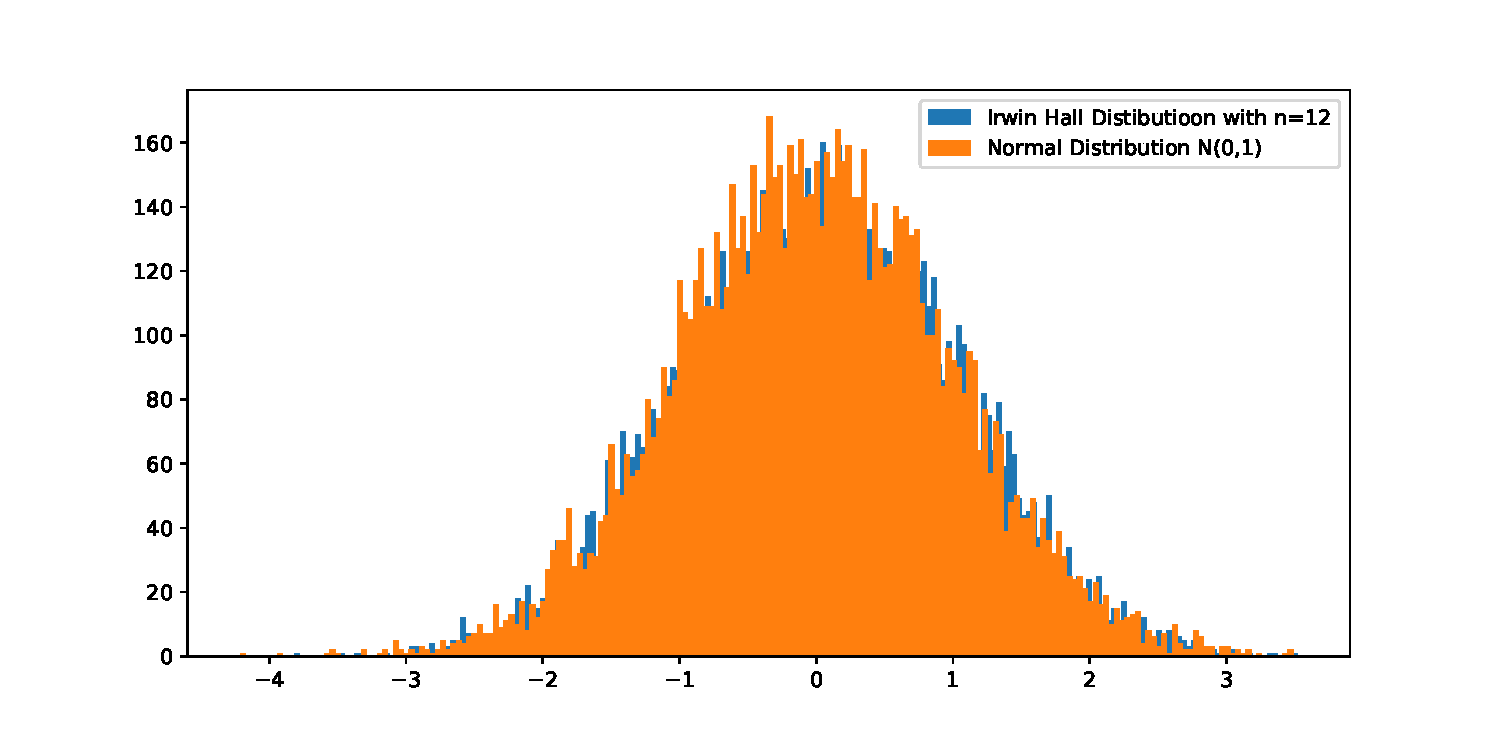
\includegraphics[width=0.8\linewidth]{numerical/figures/irwinhall}
 		\caption{}
 		\label{fig:irwinhall}
 	\end{figure}
 
 \section{Financial Instrument Pricing}
 \subsection{Black-Scholes Model}
 \begin{figure}
 	\centering
 	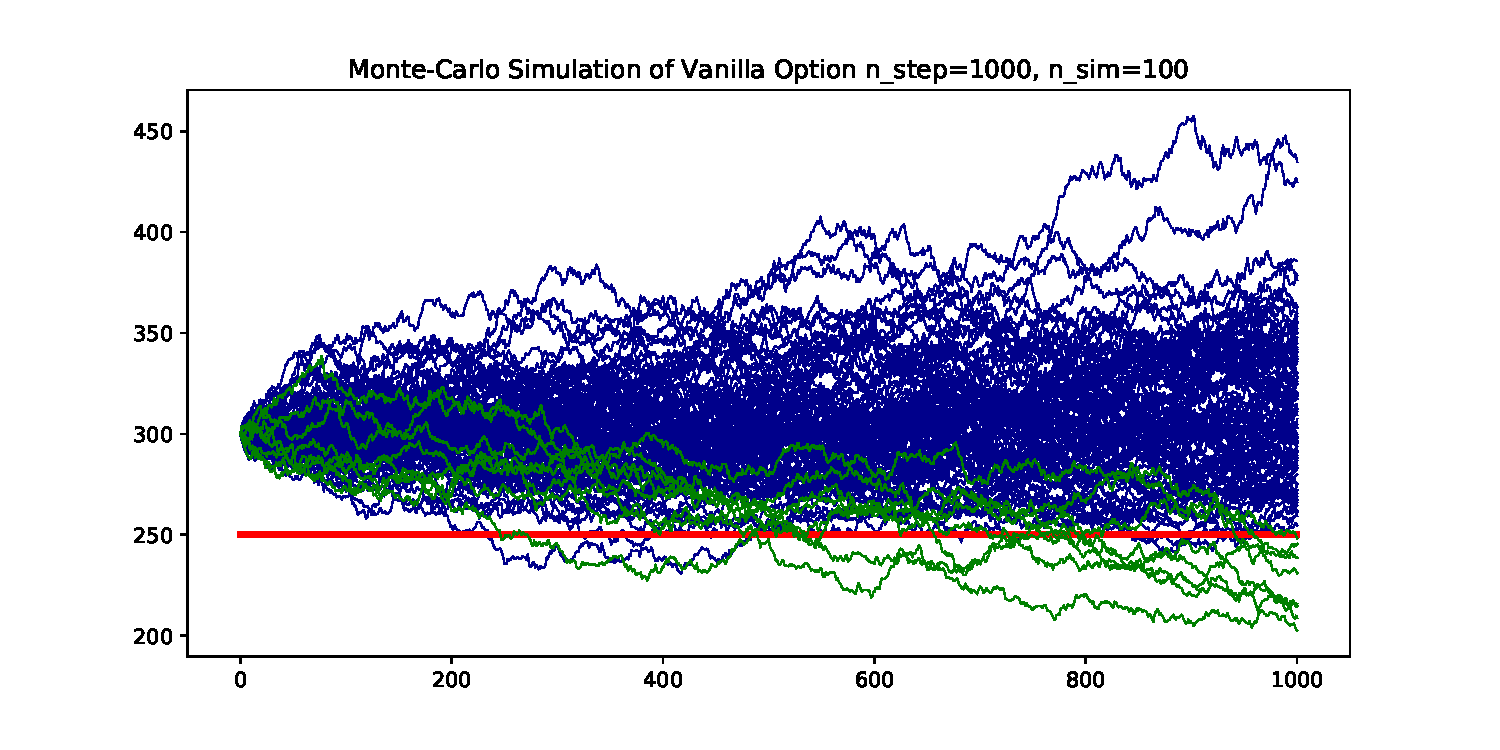
\includegraphics[width=0.8\linewidth]{numerical/figures/mcoption}
 	\caption{}
 	\label{fig:mcoption}
 \end{figure}
 
 
 
 	
\end{heur}